\documentclass[10pt,A4paper,tikz,border=20pt]{standalone}
\usepackage[utf8]{inputenc}
\usepackage[T1]{fontenc}
\usepackage{amsmath}
%\usepackage{amsfonts}
\usepackage{amssymb}
\usepackage{mathtools}
\DeclarePairedDelimiter\abs{\lvert}{\rvert}
\usepackage{tikz}
\usetikzlibrary{shapes,arrows,shapes.misc,shapes.symbols}
\usetikzlibrary{positioning}
\usepackage{gitinfo2}
\usepackage{graphicx}

\makeatletter
\AddToShipoutPictureBG{%
	\AtPageLowerLeft{%
		\kern2.6cm
		\raisebox{\dimexpr.5\paperheight-.8\height}
		{\rotatebox{90}{\gitMarkFormat\gitMarkPref{} \textbullet{} \gitMark}}%
	}%
}%
\makeatother
\newcommand{\prdfrazioni}{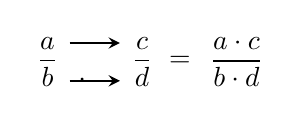
\begin{tikzpicture}[thick]
		\def\x{2.8mm}
		\def\h{2.4mm}
		\def\dist{12mm}%1cm
		\node at (0,0) {$\displaystyle \frac{a}{b}$};
		\node at (\dist,0) {$\displaystyle \frac{c}{d}$};
		\node at (1.4*\dist,0) {$\displaystyle =$};
		\node at (2.0*\dist,0) {$\displaystyle \frac{a\cdot c}{b\cdot d}$};
		% collegamento termini
		\draw[-stealth] (\x, \h)--(\dist-\x,\h); 
		\draw[-stealth] (\x,-\h)--node [near start] {$\cdot$}(\dist-\x, -\h);
	\end{tikzpicture}%
}
%\renewcommand{\gitMarkFormat}{\color{blue}\sffamily\bfseries}
\begin{document}
\tikzset{
	decision/.style={diamond, draw, %fill=blue!20,
		text width=5.5em, text badly centered, 
		node distance=3.5cm, inner sep=0pt
	},
	block/.style={rectangle, draw, %fill=blue!20,
		text width=15em, 
		text centered, 
		node distance=2.0cm,
		%rounded corners, 
		%minimum height=3em
	},
	loop/.style={chamfered rectangle,chamfered rectangle 	xsep=2cm, draw, %fill=blue!20,
		text width=15em, text centered,  
		node distance=2.5cm,% minimum height=3em
	},
	cloud/.style={draw, ellipse,%fill=red!20, 
		node distance=1.5cm, minimum height=2em
	},
	input/.style={ % requires library shapes.geometric
		draw,
		node distance=1.5cm,
			text width=15em, text centered,  
		trapezium,
		trapezium left angle=60,
		trapezium right angle=120,
	},
	line/.style={draw, very thick, %color=black!50,
		-latex'},
		print/.style={ % requires library shapes.symbols
		draw,
		text width=15em, text centered,  
		tape,
		tape bend top=none
	},
connessione/.style={
draw,
circle,
radius=5pt,
}
}
%	\begin{center}

		\begin{tikzpicture}[scale=1, %node distance = 2.5cm,
			 auto]
			% Place nodes
			\node [cloud,node distance=1cm] (init) {Inizio};
			\node [block, below of=init] (passo1) {Semplifico l'espressione};
			\node[connessione,below of=passo1] (nodo1) {};
			\node [input, below of=nodo1] (passo2) {Leggo l'espressione da sinistra verso destra cercando le incognite};
			\node [decision, below of=passo2] (decisione1) {L'incognita è a sinistra (prima) dell'uguale?};
			\node [print, below of=decisione1,node distance=3cm] (sceltasi1) {La trascrivo uguale a sinistra (prima) dell'uguale};
			\node [print, right of=decisione1,node distance=6cm] (sceltano1) {La trascrivo cambiata di segno a sinistra  (prima) dell'uguale};
			\node[connessione,below of=sceltasi1,node distance=2cm] (nodo2) {};
			\node [decision, below of=nodo2] (decisione2) {Arrivato a destra?};
			\node[connessione,below of=decisione2,node distance=2cm] (node3) {};
		\node [input, below of=node3,node distance=2cm] (passo3) {Leggo l'espressione da sinistra verso destra cercando i numeri};
		\node [decision, below of=passo3,node distance=4cm] (decisione3) {Il numero è a sinistra (prima) dell'uguale?};
	\node [print, below of=decisione3,node distance=3cm] (sceltasi3) {La trascrivo cambiato di segno a destra (dopo) dell'uguale};
\node [print, right of=decisione3,node distance=6cm] (sceltano3) {La trascrivo uguale a destra  (dopo) dell'uguale};
%			\node [cloud, below of=passo8] (fine) {Fine prodotto};

			\path [line] (init) -- (passo1);
			\path [line] (passo1) -- (nodo1);
     		\path [line] (nodo1) --  (passo2);
    		\path [line] (passo2) --  (decisione1);
     		\path [line] (decisione1) -- node[near start] {No} (sceltano1);
     		\path [line] (decisione1) -- node[near start] {Si} (sceltasi1);
			\path [line] (sceltasi1) --  (nodo2);
			\path [line] (sceltano1) |-  (nodo2);
			\path[line]  (nodo2)--(decisione2);
			\path[line] (decisione2.east)--(nodo1);
%			\path [line] (passo6) --  (passo7);
%			\path [line] (passo7) --  (passo8);
%			\path [line] (passo8) --  (fine);
		\end{tikzpicture}
%	\end{center}
\end{document}